\documentclass[../../rapport.tex]{subfiles}

\begin{document}
  Dans la théorie des types, les propositions sont des types et les preuves de ces propositions sont des éléments du type correspondant.
  Ainsi, prouver un théorème correspond à construire un élément (ou un terme) du type correspondant à l'énoncé du théorème.
  On a décrit comment construire des types de manière générale et ces constructions peuvent être utilisés pour construire des propositions,
  comme décrit dans le tableau suivant.

  \begin{figure}[ht]
    \centering
    \begin{tabular}{m{3cm} l}
      % \hline
      Logique & Type \vspace{0.4em} \\
      \hline
      \vspace{0.6em}
      $A \implies B$ & $A \fun B$ \\
      % $\forall x : A, P(x)$ & $\prod_{x:A}P(x)$ \\
      $A \wedge B$ & $A \times B$ \\
      $A \vee B$ & $A + B$ \\
      % $\exists x : A, P(x)$ & $\Sigma_{x:A}P(x)$ \\
      $\bot$ & $\0$ \\
      $\top$ & $\1$ \\
      $\neg A$ & $A \fun \0$ \vspace{0.2em}\\
      \hline \vspace{0.5em}
      $\forall x : A, P(x)$ & $\prod_{x:A}P(x)$ \\
      $\exists x : A, P(x)$ & $\sum_{x:A}P(x)$ \\
      % \hline
    \end{tabular}
  \end{figure}

  On peut donc voir les règles d'inférences comme des règles de construction des preuves dans la théorie des types.
  Par exemple, pour prouver une implication $A \implies B$, en théorie des types il faut construire une fonction $f : A \fun B$.
  Or pour construire une fonction $f$ du type $A \fun B$,
  on doit donner une manière de construire une preuve de $B$ à partir d'une preuve de $A$,
  c'est-à-dire que si $a : A$ est un preuve de $A$, $f\ a$ est une preuve de $B$ et ce pour toute preuve $a$ de $A$.
  On peut alors voir la fonction $f$ comme un algorithme qui donne une preuve de $B$ à partir de n'importe quelle preuve de $A$.

  Ainsi, les règles d'introduction des types donnent une manière de construire des éléments du type en question,
  et donc si ce type représente une proposition alors on peut voir la règle d'introduction comme une règle de construction de preuve.
  De la même manière les règles d'élimination donnent la manière d'utiliser une hypothèse.

  Enfin, les deux derniers types du tableau sont les quantificateurs universels et existentiels et leurs équivalents : les types dépendants.
  Le caractère dépendant de ces types se situe dans le fait qu'ils dépendent d'un paramètre :
  pour les fonctions dépendantes le codomaine dépend du point d'application,
  pour les paires dépendantes c'est le type de la deuxième coordonnées qui dépend de la première coordonnée.
  Le caractère dépendant de ces types permet notamment la construction de polymorphismes,
  comme détaillé dans la section sur les fonctions dépendantes.

  % Si on considére $A : \U_i$ et $B : A \fun \U_i$, un élément $f$ du type $\prod_{a: A}B(a)$ associe à un élément $a : A$
  % une preuve de $B(a)$, le type $A$ est donc un type d'éléments alors que $B$ est un prédicat sur le type $A$.
  %
  % De même, un élément $(a, b)$ du type $\sum_{a:A}B(a)$ est donc constitué d'un élément $a : A$ et d'une preuve $b$ de $B(a)$.
  % Or pour prouver l'existence d'un élément $a : A$ vérifiant le prédicat $B$, il faut à la fois fournir l'élément qui vérifie $B$
  % et un preuve que cet élément vérifie le prédicat $B$, \textit{ie.} un élément de type $\sum_{a:A}B(a)$.

  \vspace{1em}
  Prouver une proposition en théorie des types est équivalent à construire un élément d'un certain type.
  Pour ce faire, les assistants de preuves permettent de simplifier la création de terme (ou d'éléments).
  Par exemple, la proposition
  $$(\neg (p \wedge q) \implies r) \implies (\neg p \implies r) \wedge (\neg q \implies r).$$
  correspond au type
  \begin{align*}
    &(\neg (p \times q) \fun r) \fun (\neg p \fun r) \times (\neg q \fun r) \\
    \equiv\ &(((p \times q) \fun \0) \fun r) \fun ((p \fun \0) \fun r) \times ((q \fun \0) \fun r).
  \end{align*}
  dont un terme est
  $$
  \lambda h.\ (\lambda x.\ h\ (\lambda a.\ x\ (\pi_1\ a)), \lambda y.\ h\ (\lambda a.\ y\ (\pi_2\ a)))
  $$
  En effet si on considère $h : ((p \times q) \fun \0) \fun r$,
  pour construire un terme de type $(p \fun \0) \fun r$ (\textit{resp}. $(q \fun \0) \fun r$),
  on se donne $x : p \fun \0$ (\textit{resp}. $y : q \fun \0$),
  puis on cherche à construire un terme de type $r$ dans les deux cas.
  Pour ce faire, on applique la fonction $h$ à un terme du type $(p \times q) \fun \0$ que l'on doit construire.
  Or, $\pi_1\ a$ (\textit{resp.} $\pi_2\ a$) est de type $p$ (\textit{resp.} $q$) si $a$ est de type $p \times q$,
  donc $x\ (\pi_1\ a)$ (\textit{resp.} $y\ (\pi_2\ a)$) est de type $\0$.
  Les fonctions $\lambda a.\ x\ (\pi_1\ a)$ et $\lambda a.\ y\ (\pi_2\ a)$ sont de type $p \times q \fun \0$,
  on peut alors appliquer $h$ à chacune de ses deux fonctions pour obtenir un terme de type $r$ comme voulu.

  La construction d'une telle fonction est parfois compliquée, c'est pourquoi les assistants de preuves possèdent
  un système de construction de termes à partir de commande plus simple ayant un sens qui se rapproche des règles habituelles
  de raisonnement.
  Reprenons l'exemple précédent. En Lean, le code suivant qui permet de construire un terme de ce type :
  % \begin{figure}[ht]
  %   \centering
  %   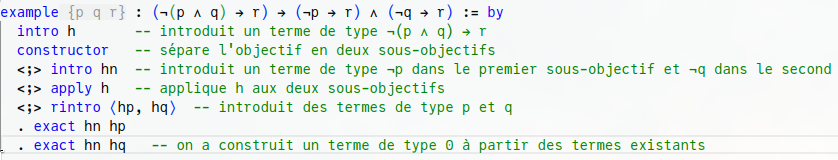
\includegraphics[width=0.95\textwidth]{lean.png}
  % \end{figure}
  \begin{lean4code}
    example : (¬(p |$\wedge$| q) → r) → (¬p → r) |$\wedge$| (¬q → r) := by
      intro h 	    -- Introduit un terme de type ¬(p |$\wedge$| q) → r)
      constructor 	-- Sépare l'objectif en deux sous-objectifs
      <;> intro hn        -- Introduit un terme de type ¬p (resp. ¬q)
                          -- dans le premier (resp. second) sous-objectif
      <;> apply h 	-- Applique h aux deux sous-objectifs
      <;> rintro ⟨hp, hq⟩ -- Introduit des termes de type p et q
      . exact hn hp
      . exact hn hq       -- Construit des termes de type 0
  \end{lean4code}
  Le terme créé par Lean à partir de ce code est :
  \begin{lean4code}
    fun h =>
      ⟨fun hn => h fun a => And.casesOn a fun hp hq => hn hp,
       fun hn => h fun a => And.casesOn a fun hp hq => hn hq⟩
  \end{lean4code}

\end{document}
